\section{Durchführung}
Der Versuch wird mit einem TeachSpin Quantum Analog System durchgeführt, welches in den Abbildungen
(\ref{pic:1}) und (\ref{pic:2}) dargestellt ist. Dabei werden an die Röhrenkonstruktion ein Mikrofon und ein Lautsprecher
angeschlossen, welche über den Controller (Abbildung \ref{pic:2}) mit einem Laptop verbunden sind. Hiermit lässt
sich nun die Schallamplitude in Abhängigkeit von der Frequenz messen. Vor Beginn der Messungen werden Mikrofon und Lautsprecher am
Controller und am Laptop so einjustiert, dass ein optimales Signal aufgenommen werden kann.

\begin{figure}[H]
  \centering
  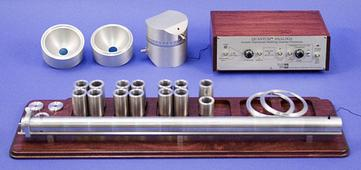
\includegraphics[scale=.75]{pic1.jpg}
  \caption{Aufbau des TeachSpin Quantum Analog System.} \cite{durch1}
\end{figure}

\begin{figure}[H]
  \centering
  
\includegraphics[scale=.75]{pic2.png}
  \caption{Benutzeroberfläche des TeachSpin Quantum Analog Controllers.} \cite{durch1}
\end{figure}

\subsection{Teilchen in einem periodischen Potential}
Zunächst wird die Analogie zu einem Teilchen in einem periodischen Potential untersucht.  \\
\newline
\noindent
Als erstes werden Frequenzspektren für die Rohrlängen @@, @@ und @@ in einem Bereich von \SI{0.1-10}{\kilo\hertz} aufgenommen, und für \SI{12 x 50}{\milli\meter} bei \SI{0.4-12}{\kilo\hertz}. \\
\newline
\noindent
Dann werden drei Spektren bei einer Länge von \SI{8 x 50}{\milli\meter} im Bereich \SI{0.4-12}{\kilo\hertz} aufgenommen, jeweils mit 10, 13 und \SI{16}{\milli\meter} Linsen zwischen den Röhren.
Eine Linse ist hier eine schmale Scheibe mit einem geringeren Durchmesser als die Röhren.
Das Gleiche wird für eine Länge von \SI{10x 50}{\milli\meter}, \SI{12 x 50}{\milli\meter} und \SI{8 x 75}{\milli\meter}, je getrennt von \SI{16}{\milli\meter} Linsen, durchgeführt. \\

\subsection{Modell der Bandstruktur eines Festkörpers}
Nun wird die Analogie zu einem Teilchen, welches sich in der Bandstruktur eines Festkörpers befindet, betrachtet. \\
\newline
\noindent
Zu Beginn wird das Spektrum einer \SI{50}{\milli\meter}, und einer \SI{75}{\milli\meter} Röhre im Bereich \SI{0.4-22}{\kilo\hertz} aufgenommen. \\
Anschließend werden \SI{2 x 50}{\milli\meter} Röhren im Bereich \SI{0.4-12}{\kilo\hertz} untersucht, je mit 10, 13 und \SI{16}{\milli\meter} Linsen zwischen ihnen. \\
Nun werden sogenannte Einheitszellen gebildet, bestehend aus jeweils einer Röhre und einer Linse. Nacheinander werden die Spektren von 3, 4 und 6 Einheitszellen im Bereich
\SI{0.4-12}{\kilo\hertz} gemessen, jeweils für alle drei Linsengrößen. \\
Derselbe Bereich wird mit \SI{12 x 50}{\milli\meter} Röhren untersucht, wobei diese nun abwechselnd von 13, und \SI{16}{\milli\meter} Linsen getrennt sind.\\
Dann werden 5 Einheitszellen im selben Bereich vermessen, bestehend aus jeweils einer \SI{50}{\milli\meter}, einer \SI{16}{\milli\meter} Linse, einer \SI{75}{\milli\meter} Röhre und einer weiteren \SI{16}{\milli\meter} Linse. \\
Als nächstes werden \SI{12 x 50}{\milli\meter}, getrennt von \SI{16}{\milli\meter} Linsen, aufgebaut. Es wird nun eine Röhre an letzter Stelle durch eine Röhre der Länge \SI{12.5}{\milli\meter}, dann eine an Stelle 2 durch eine \SI{25}{\milli\meter} Röhre,
eine an Stelle 9 durch eine \SI{37.5}{\milli\meter} Röhre, eine an Stelle 7 durch eine \SI{75}{\milli\meter} Röhre und eine an letzter Stelle durch eine \SI{75}{\milli\meter} Röhre. 
Hierbei sind die Stellen von dem Mikrofon ausgehend zu zählen und zwischen einem Austausch wird die ursprüngliche Anordnung wieder aufgebaut.



% Quelle: http://www.teachspin.com/quantum-analogs.html
% mit Name "durch1"
